\section{Building Why3 plugins} % approx. 5 pages

\subsection{Interface} % approx. 2 pages

The interface items required for creating a plugin
are part of the publicly exposed Why3 API.
This has some introductory documentation, %TODO: point towards docs chapter
but much of the API is only documented insofar as it is exposed in header files.
The modules of primary interest to us are part of the \inl{core} modules
(aptly located in \inl{<WHY3>/src/core/}):
\begin{itemize}
    \item \inl{Env}: Language registration.
    \item \inl{Theory}: Theories (core language).
    \item \inl{Decl}: Declarations (theory components).
    \item \inl{Term}: Logic formulas.
    \item \inl{Ty}: Types.
    \item \inl{Ident}: Identifiers.
\end{itemize}

% Plugin architecture
Why3 accepts plugins in the form of dynamically loaded executables.
At startup, Why3 executes specified plugin binaries
such that they may register languages, formats, printers, parsers, and transformations.

\begin{figure}[H]
    \center
    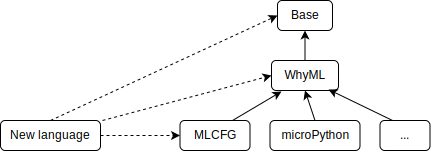
\includegraphics[width=0.5\textwidth]{figs/language_tree.pdf}
    \caption{The default Why3 language tree. \label{fig:langtree}}
\end{figure}

Why3 tracks supported languages in a tree.
Using \inl{Env.register\_language},
plugins can register any arbitrary type as a language
by providing a conversion function to an already-existing language in the tree.
There are two built-in languages that may be targeted for conversion:

\begin{itemize}
    \item \inl{Env.base\_language : Theory.theory Wstdlib.Mstr.t language}\\
          The base language, a dictionary of \inl{theory} values.
    \item \inl{Pmodule.mlw\_language : Pmodule.mlw\_file language}\\
          An internal representation of the WhyML/MLW language.
\end{itemize}

The choice of conversion target depends on our goal.
If the new language can be converted to a WhyML or MLCFG syntax tree,
this will generally be the easier route,
as we can then leverage the power of the existing verification condition generators.
If the language has novel features that require unique VC generation,
we can implement this as a conversion from our language to a theory.
In this project we target the base language,
as this allows us to see how we can use the Why3 framework to build custom VC generators.

Using \inl{Env.register\_format} with a parser and a language handle,
we can register new textual formats for any language.
In fact, the built-in plugins only register new textual formats for MLW.
This is sufficient for most smaller languages such as our While-lang,
but it doesn't create an entry in the language tree,
so a novel language registered this way cannot be a conversion target.

\subsection{Creating formulas}

Logical formulas in Why3 are represented by encapsulated \inl{term} objects,
and are created and modified using combinators from the \inl{Term} module.
The combinators include various constants, predicate logic, function applications,
variable substitutions, and more.
For example, we can create the formula
$\forall x y.~(x \rightarrow y) \leftrightarrow (\neg x \lor y)$
as follows:
\begin{lstlisting}
open Why3
open Term
open Ident

let x     = create_vsymbol (id_fresh "x") in
let y     = create_vsymbol (id_fresh "y") in
let x_var = t_var x in
let y_var = t_var y in
let t1    = t_implies x_var y_var in
let t2    = t_or (t_not x_var) y_var in
let t     = t_forall_close [x; y] [] (t_iff t1 t2)
\end{lstlisting}

Note that identifiers are created using \inl{id\_fresh},
which always creates a unique identifiers.
In order to use the same variable multiple times,
it's necessary to use the exact same identifier every time.

Terms and identifiers can also be annotated with locations and attributes using
\inl{Term.t\_set\_attr}.
Position annotations are what enables the Why3 IDE to highlight goals
and subdivided goals after splits.

\subsection{Declarations}

Declarations are made using builder functions located in the module \inl{Term}.
A declaration can be one of:

\begin{itemize}
    \item Abstract types and type aliases
    \item Algebraic data types
    \item Abstract functions and predicates
    \item Defined functions and predicates
    \item Inductive predicates
    \item Propositions:
    \begin{itemize}
        \item Axioms
        \item Lemmas
        \item Goals
    \end{itemize}
\end{itemize}

Theories are primarily built from declarations.
Our small language will translate into a theory with a single goal proposition.

\subsection{Building a \inl{theory}}

All languages are eventually translated into to the base language,
a dictionary of \inl{theory} objects.
A \inl{theory} object is an intermediate representation of a module.
This is the core representation that Why3 can apply transformations to,
convert to SMT queries, and extract code from.

The \inl{theory} type is provided by the \inl{Theory} module,
located in \inl{src/core/theory.mli}.
Theories are created using an encapsulated builder pattern.
Theories ``under construction'' are  created with \inl{create\_theory},
modified using transformers such as \inl{add\_decl},
and finalized using \inl{close\_theory}.

\subsection{Printing}

In addition to parsing,
it is also possible to register a printer for a set of core objects.
This is useful for presenting formulas and tasks in a way that match the syntax of our language.
This is not a strict requirement.
